\section{Description}

In this section we will looking the device more detailed and give the description of all the parts used in the system.

For the reaction wheel we are using a brushless DC motor from maxon EC 45 flat 50W.
We chose a brushless DC motor because it has less friction and therefore we have less energy going to waste.
The particular motor was chosen for its performance specifications.
The main criteria was to find a motor with enough torque for our system.
(All the values used onwards in this project are taken from the datasheets or are the assuming values of the physical details what would be used in the prototype.)
As we can see from the datasheet the maximal continious torque on that motor is 83.4 nNm what is sufficient for our system.
It also has high maximum rpm which is 6710.
In our first model and culations we determined that the speed needed to jump the cube 
\begin{equation}
 \Delta E=mg\Delta h
\end{equation}
\begin{equation}
 \Delta E=\frac{1}{2}I\omega ^{2}
\end{equation}
\begin{equation}
 \frac{1}{2}I\omega ^{2}=mg\Delta h
\end{equation}
\begin{equation}
 I=m_{w}r^{2}
\end{equation}
\begin{equation}
 mg\Delta h=\frac{1}{2}m_{w}r^{2}\omega ^{2}
\end{equation}
\begin{equation}
 \omega ^{2}=2\frac{mg\Delta h}{m_{w}r^{2}}
\end{equation}

Where $m$ is the mass of the whole system, $g$ is the gravitational acceleration, $\Delta h$ is the height differents of the two mass centres in diffetent stable positions.
$m_{w}$ is the mass of the reaction wheel and $r$ is the radius of the wheel.

When we insert our initial values of the device, what we designed we get the rotational speed approximately 289 rpm.
As we can see the motor is more than sufficient to make the cube jump.

The motor is controlled by a Maxon escon 36/3 EC servo controller driver.
This driver was chosen because of the compatibility with the motor.
On this patricular driver it is possible to control the motor with current control or speed control.
In our system it is vital that we can control the motor by current control because $ T_{m}(t)=K_{m}u(t)$ as we can see the torque, what is our main input to control, is what we need to manipulate.

To break the wheel we have built a breaking system with a servo motor Hitec HS-485HB.
The breaking of the wheel is crucial in the jumping sequence to convert the wheels rotational energy into the potential energy of the whole body.
Breaking is done by physically constricting the wheel which the servo.

While balancing the system we use the torque of the wheel to move its angle.
For determining the position of the wheel we have mounted an accelerometer on the device.
The accelerometer is MPU-6050.
We are using the Earths gravitational accelerations projection on the vertical axes of the body to get the off-set angle.
%insert pic with offset angle and gravity vector
\begin{figure}[H]

	
	\centering
 	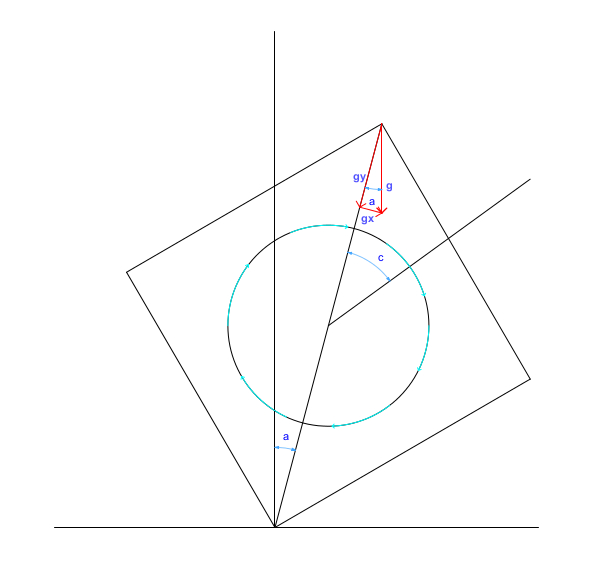
\includegraphics[width=1\textwidth]{images/kuubik1crop2.jpg}
	
	~
	\caption{Cube offset angles and gravity vector} 
 	\label{fig:mech} 
\end{figure}

In the figure above c is later used as $\theta_{w}$ and a is used as $\theta_{b}$.


Body of the device is a square plate made out of aluminium.
We have cavities in the plate because it makes the system less heavy and therefore we need less force to move it as we desire.
On the square plate are mounted the reaction wheel made from the BLDC and a aluminium circle.
Furthermore the breaking servo is mounted near the bottom bearing of the system.
When the system is in the balancing point then on the top most corner is mounted the accelerometer.
%insert picture of the whole system

